\documentclass[fleqn,10pt]{wlscirep} 

\usepackage{setspace}
\usepackage{lineno}
\doublespacing


%%%% (20 words or less)
\title{Genotypic variation in a foundatio tree drives ecological network structure}


\author[1,2,*]{Matthew K. Lau}
\author[2]{Louis J. Lamit}
\author[3]{Rikke R. Naesbourg}
\author[4]{Stuart R. Borrett}
\author[5]{Matthew A. Bowker}
\author[1]{Thomas G. Whitham}

\affil[1]{Department of Biological Sciences and Merriam-Powell Center
  for Environmental Research, Northern Arizona University, Flagstaff,
  AZ 86011, USA}
\affil[2]{Harvard Forest, Harvard University, 324 N Main St,
  Petersham, MA 01366, USA}
\affil[3]{University of California Berkeley, Berkeley, CA, USA}
\affil[4]{Department of Biology and Marine Biology, University of
  North Carolina Wilmington, 601 South College Road, Wilmington, NC,
  28403, USA}
\affil[5]{School of Forestry, Northern Arizona University, Flagstaff,
  AZ 86011, USA}


\affil[*]{matthewklau@fas.harvard.edu}

%% \affil[+]{these authors contributed equally to this work}

\keywords{Keyword1, Keyword2, Keyword3}

\begin{abstract}

Biological evolution is argued to occur in the context of complex
networks of interacting species in which natural selection defines the
structure of ecological networks \cite{Rezende2007, Guimaraes2011,
  Moya-Larano2011, Thompson2014, Fortin2017}. However, fundamental to
this evolutionary process is the discovery of a genetic basis to
ecological network structure, which remains largely unknown.  Here, we
use both a long-term experimental common garden \cite{Martinsen2001}
with genotyped individuals and a natural riparian forest of the
foundation tree species \cite{Ellison2005} \textit{Populus
  angustifolia}, to test how genetic variation contributes to the
interaction network structure of a model community comprised of
epiphytic lichens. We found three main results:  1) lichen communities
showed significant unipartite (i.e., one mode) network structure that
was similar between the common garden and a natural stand, 2)
individual tree genotype significantly influenced lichen species
interactions, which was strongly correlated with bark roughness, a
genetically based trait in cottonwoods \cite{Ying1976} known to
influence epiphytic lichen \cite{Lamit2011}, and 3) bipartite (two
mode) genotype-species networks, comprised of the foundation species
and its associated lichen community, showed significant modular
structure in both the common garden and natural stand. In
demonstrating a strong genetic component to ecological network
structure, selection differentially acting on different tree genotypes
will likely alter network structure and vice-versa, selection acting
on the network in a community context could feed back to affect plant
performance and evolution.  Such findings set the stage for
quantifying community evolution and the evolution of Darwin’s
‘entangled bank’, a metaphor that characterizes the complexity and
interconnectedness of complex communities in nature.

\end{abstract}

\begin{document}

\flushbottom
\maketitle
% * <john.hammersley@gmail.com> 2015-02-09T12:07:31.197Z:
%
%  Click the title above to edit the author information and abstract
%
% ^ <thomas.whitham@nau.edu> 2018-03-02T21:05:44.603Z.
\thispagestyle{empty}

%% \noindent Please note: Abbreviations should be introduced at the
%% first mention in the main text – no abbreviations lists. Suggested
%% structure of main text (not enforced) is provided below.

\linenumbers

%%% For Submission to Nature Ecology and Evolution %%%
%%% https://www.nature.com/natecolevol/info


\section*{Introduction}

Evolution occurs in the context of complex networks of interacting
species. In ecological communities, community dynamics depend on key
interactions \cite{Fontaine2011} that occur in species interaction
networks, such as:  trophic \cite{Bascompte2006} and mutualistic
\cite{Rafferty2013} interaction networks. Phylogenetic patterns in
ecological networks support the importance of evolutionary processes
in shaping species interactions, community structure and ecosystem
processes \cite{Crutsinger 2016, Rezende2007, Whitham2006a}. Community
genetics studies \cite{Lamit et al. 2015} have shown that genetic
variation in foundation species \cite{Ellison2005} plays a significant
role in defining distinct communities of interacting organisms:  such
as, endophytes, pathogens, lichens, arthropods, and soil
microbes. Multiple studies have now demonstrated that genetic
variation influences numerous functional traits (e.g., phytochemical,
phenological, morphological) produces a multivariate phenotype
\cite{holeski2012} tha contributes to variation in associated
communities \cite{Bailey2009a}. Additional work has provided support
for the hypothesis that not only does composition vary among
genetically distinct genotypes of foundation species but it also
impacts the structure of the network of species interactions in these
communities \cite{Keith2017, Lau2016}.


\textbf{Network structure is important for evolutionary dynamics}

Bascompte et al. 

Rezende

Andreazzi, C.S, J. N. Thompson, and P. R. Guimarães, Jr. 2017. Network
structure and selection asymmetry drive coevolution in species-rich
antagonistic interactions. American Naturalist 190:99-115

Toju, H. M. Yamamichi, P. R. Guimarães, Jr., J. M. Olesen, A. Mougi,
T. Yoshida, and J. N. Thompson. 2017. Species-rich networks and
eco-evolutionary synthesis at the metacommunity level. Nature Ecology
and Evolution 1:0024. DOI: 10.1038/s41559-016-0024

Dáttilo, W., N. Lara-Rodriguez, P. Jordano, P. R. Guimarães, Jr.,
J. N. Thompson, R. J. Marquis, L. P. Medeiros, R. Ortiz-Pulido,
M. A. Marcos-García, and V. Rico-Gray. 2016. Unraveling Darwin's
entangled bank: architecture and robustness of mutualistic networks
with multiple interaction types. Proceedings of the Royal Society B
283: 20161564.


\textbf{Foundation species impact ecological networks}

Toju, H., P. R. Guimarães, Jr., J. M. Olesen, and
J. N. Thompson. 2015. Plant communities and below-ground plant-fungal
networks. Sciences Advances 1:e1500291

Toju, H., P. R. Guimarães, Jr., J. M. Olesen, and J. N. Thompson. 2014
Assembly of complex plant-fungal networks. Nature Communications
5:5273 DOI:10.1038/ncomms6273

Guimarães, P. R., Jr., P. Jordano, and J. N. Thompson. 2011. Evolution
and coevolution in mutualistic networks. Ecology Letters 14:877-885.

Cuautle, M., and J. N. Thompson. 2010. Evaluating the co-polliinator
network structure of two sympatric Lithophragma species with different
morphology. Oecologia 162:71-80.

Díaz-Castelazo, C., P. R. Guimarães, Jr., P. Jordano, J. N. Thompson,
R. J. Marquis, and V. Rico-Gray. 2010. Changes of a mutualistic
network over time: reanalysis over a 10-year period. Ecology
91:793-801.

Guimarães, P. R., Jr., V. Rico-Gray, P.S. Oliveira, T. J. Izzo,
S. F. dos Reis, and J. N. Thompson. 2007. Interaction intimacy affects
structure and coevolutionary dynamics in mutualistic networks. Current
Biology 17:1797-1803

Guimarães, P.R., V. Rico-Gray, S.F. dos Reis and J.N. Thompson
(2006). Asymmetries in specialization in ant–plant mutualistic
networks. Proc. R. Soc. B 273: 2041–2047.


\textbf{Foundation species genetics matters to communities and ecosystems}

Genetic variation of a foundation rockweed species affects associated
communities Jormalainen et al September 2017 Ecology

A geographic mosaic of genetic variation within a foundation tree
species and its community‐level consequences
Robert C. Barbour  Julianne M. O'Reilly-Wapstra  David W. De Little
Gregory J. Jordan Dorothy A. Steane  Jonathon R. Humphreys  Joseph
K. Bailey  Thomas G. Whitham  Bradley M. Potts

Ghering 2017: Tree genetics defines fungal partner communities
  that may confer drought tolerance


Jamie's recent paper

Hughes et al.

Leroy et al

Crutsinger, G.M., 2016 A community genetics perspective: opportunities
for the coming decade. New Phytologist, 210, 65-70.

Nat Eco Evo 2017



\textbf{Genetic basis of networks}

Fortuna et al. 2009

Daves 2016 paper

Keith, A.R., J.K. Bailey, M.K. Lau, and T.G. Whitham.  2017.
Genetics-based interactions of foundation species affect community
diversity, stability, and network structure.  Proceedings of the Royal
Society B 284: 20162703. http://dx.doi.org/10.1098/rspb.2016.2703.

Lamit, L.J., P.E. Busby, M.K. Lau, Z.G. Compson, T. Wojtowicz,
A.R. Keith, M.S. Zinkgraf, J.A. Schweitzer, S.M. Shuster,
C.A. Gehring, and T.G. Whitham.  2015.  Tree genotype mediates
covariance among diverse communities from microbes to arthropods.
Journal of Ecology 103:840–850.

Lau, M.K., A.R. Keith, S.R. Borrett, S.M. Shuster, and T.G. Whitham.
2016.  Genotypic variation in foundation species generates network
structure that may drive community dynamics and evolution.  Ecology
97:733-742.


None of the community genetics network papers have looked at
species-species newtorks of associated organisms.


Here, we investigate how genetic variation in a foundation tree
species determines the structure of a network of interactions among a
community of lichen species. Using a long-term (20 years+), common
garden experiment with replicated individuals of known genetic
identity and a naturally established stand of
\textit{P. angustifolia}. We focused on a model community of 9
epiphytic lichens species, as previous research has demonstrated
significant compositional responses of epiphytes to genotypic
variation \cite{Winfree2011, Zytynska2011}. In addition, the
life-history characteristics of lichen, having highly localized,
direct contact interactions and slow population turnover rates,
allowed us to assess interactions among lichen species on individual
trees. We hypothesize that in natural systems evolution occurs in a
community context involving interactions of complex networks of
interacting species \cite{Keith et al. 2017, Thompson2013,
  Bascompte2007, Darwin1855}.  If correct, we should expect to find
that network structure is genetically based in which different plant
genotypes support different interaction networks and that these
interactions networks can function as indicators of ecological
dynamics important for conserving biodiversity.  Applying a dual-scale
(lichen-lichen and genotype-lichen interactions) }network analysis
  approach, we then examined the genetically based impacts of
  \textit{P. angustifolia} on network structure.

%% Topical subheadings are allowed. Authors must ensure that their
%% Methods section includes adequate experimental and characterization
%% data necessary for others in the field to reproduce their work.

\section*{Results}

%%% Up to three levels of \textbf{subheading} are permitted. Subheadings should not be numbered.

\subsection*{Tree Genotype Influences Ecological Network Structure}

In both the experimental garden and the natural stand, we discovered
that genotypic variation in a \textit{P. angustifolia} predictably
influenced the structure of the lichen species interaction network and
contributed to the formation of evolutionary modules comprised of tree
genotypes and the lichen community.  We focused our network analysis
on modularity (i.e. the formation of compartments) and nestedness
(i.e. the overlap in sets of interactions among species) both of which
are of interest in the context of the interplay between ecological and
evolutionary dynamics as have established theoretical and empirical
support as relevant structural metrics of ecological dynamics and can
serve as indicators of the units of evolution in a community context.
We observed significant unipartite (one-mode) network structure
\cite{Araujo2011} in the lichen species interaction networks that was
similar between the experimental garden and the natural stand (Fig. 1a
and 1b; Garden: z = -6.31, p = 0.0002; Natural: z = -3.15, p =
0.002). The two networks displayed high multivariate structural
similarity (Mantel R = 0.51, p = 0.029).

Node level eigen-centrality \cite{DeAngelis1989}, a measure of species
importance that integrates indirect connections, showed strong
correlation between the two stands (Fig. 1c; r = 0.7, t = 2.6135, df =
7, p = 0.035). Centrality was also highly correlated with total
abundance in both networks (Fig. 1d; Garden: r = 0.77, t = 3.2427, df
= 7, p = 0.014; Natural:  r = 0.86, t = 4.43, df = 7, p = 0.003). In
combination, the similarity of both the whole and node level network
structure between the common garden and the wild indicates that the
common garden environment captures much of the natural variation that
exists in nature and accurately reflects natural processes.

\subsection*{Network Response to Tree Trait Variation}

In the common garden, where the effect of environmental variation was
controlled, genotype was an important factor contributing to network
structure. Genotype was a significant predictor of interactions on
individual trees (Fig. 2a; F = 3.4213, num df = 12.000, denom df =
14.668, p-value = 0.01426). Similar to the effect of a genetically
controlled trait (bark roughness) on a dominant lichen
\cite{Ellison2005}, we found that individual tree genotypes with
similar levels of bark roughness had similar levels of lichen
interactions (Fig. 2a; Mantel R = 0.08, p = 0.013), which was similar
to the correlation observed between bark roughness and lichen
interactions in the natural stands (Fig 2b: r = -0.53, p = 0.050).


\subsection*{Genetic Structure Generates Foret-Scale Network Structure}

We also examined how \textit{P. angustifolia} genotypic
differentiation contributes to the formation of groups of tree
genotypes and lichen species and found significant modular
structure. Using a bipartite (two-mode) network approach in which
genotype-species networks were modeled using the species maximum
relativized values of each lichen species across all
\textit{P. angustifolia} genotypes, we found significant modularity in
the common garden stand (Fig. 3a; z = 9.64, p < 0.001). When using the
same analyses on individual trees in the natural stand, we also found
significant modularity (Fig. 3b; z = 7.42, p < 0.001). Furthermore,
nestedness of both of these networks was significantly lower than
expected under a null model (Garden: z = -2.30, p < 0.001; Natural
Stand: z = -2.84, p < 0.001), most likely as a result of module
formation.



\section*{Discussion}

%%% The Discussion should be succinct and must not contain subheadings.

These findings support the hypothesis that genotypic variation in a
foundation species contributes to the structure of a network of
interacting species that might be least expected to exhibit such
structure. 

\textbf{TGW: MIGHT BE GOOD TO CITE PAPERS ON COMEPTITION IN LICHENS OR
OTHER ORGANIZING FACTORS TO BACK UP THE LEAST EXPECTED STATEMENT.  AS
EPIPHYTES WE MIGHT NOT EXPECT THEM TO CARE.}

\textbf{MKL: This is a job for Lamit and Rikke.}

Several lines of evidence support this conclusion. First, the wild
stand showed significant interaction network structure (Fig. 1a and
b); and both tree genotype and the genetically based tree trait, bark
roughness, was a strong predictor of co-occurrence patterns
(Fig. 2a). 

\textbf{TGW: I THINK WE NEED TO EMPHASIZE THE LONG-TERM NATURE OF OUR
COMMON GARDEN STUDY AS VERY FEW COMMON GARDEN STUDIES OF LICHENS
LIKELY EXIST. ANY REFS ON THIS? IF TRUE MIGHT WANT TO MENTION THIS UP
FRONT IN INTRO.}

\textbf{MKL: Same here. This is a job for Lamit and Rikke.}

Second, in a long-term common garden study, network
(Fig. 1b) structure showed a high degree of similarity to the wild
stand network structure (Fig. 1c and d). Third, tree genotype was a
significant predictor of SES values (Fig. 2a), displaying significant
correlation with a genetically linked trait, bark roughness, both in
the common garden (Fig. 2a) and in a naturally established stand of
trees (Fig. 2b). Last, both of the bipartite genotype-species networks
in the common garden and natural stand displayed significant
modularity, suggesting that genotypic variation is leading to the
formation of evolutionarily dynamic compartments within the
community. Thus, just as numerous studies have shown that plant
genotype can affect species richness, abundance, diversity, and
composition and previous work has demonstrated that evolutionary
processes shape ecological networks \cite{Guimaraes2011,
  Moya-Larano2011}, our study includes genetics in an empirical
investigation that combines both experimental common garden findings
along with studies in the wild that are in close agreement.

Our results point to the importance of understanding the community
level effects of genetic variation and corroborate previous findings
of the importance of plant genetics in shaping community structure and
ecosystem processes \cite{Whitham2006a}.  This study highlights the
potential for indirect effects of genetic variation to propagate
through networks of interacting species and trophic levels. Altering
the structure of interaction networks presents a means for genetic
effects to be magnified within the system of interacting species. For
example, Keith et al. (2017) showed that the genetics based
interations of aphid resistant and aphid susceptible trees resulted in
different interaction networks of their associated arthropod
communities composed of 139 species. At the scale of ecosystems,
trophic networks or food webs direct and control the rates of energy
and nutrient flux \cite{Borgatti2006}. Furthermore, in a
predator-prey-plant study, Smith \cite{Smith2011}, showed that the
interactions among species across trophic levels depended on plant
genotype.

Tylianakis 2010 Conservation of species interaction networks.

\begin{itemize}
\item Functions-Metrics (Figure 2: 
  \begin{itemize}
  \item Richness/Connectance = Increased function and function
    stability
  \item Nestedness = Buffer extinctions in mutualistic networks
  \item Compartmentalization = greater stability, slow spread of
    disturbance (i.e. trophic cascades)
  \item Proportion of Weak Links = stability, fewer cascades
  \item Connectivity Distribution = Indicate Assembly, Robustness to
    2nd extinctions
  \end{itemize}
\item Focus on metrics that saturate quickly with sampling
\item Connectivity, Compartmentalization, Nestedness
\item Need more research on the impacts of perturbations on these
  networks
\end{itemize}



\begin{itemize}
\item Networks working at multiple scales re-inforce connectivity
\item Gene networks (Zink)
\item Community networks (Keith2017, Lau 2016)
\item Stand scale (This work)
\item Landscape scale (Bothwell2017)
\end{itemize}

Although our study was conducted with a community of lichens, these
results should be generalized to other groups of diverse organisms
around the world that also exhibit significant genetic signals at the
community level \cite{Rowntree2011, Whitham2012}, although spatial
scale of interactions should be considered \cite{Zook2010} Bangert et
al. 2006. As heritable variation is the raw material for natural
selection to act upon, a genetic basis for interaction network
structure indicates evolutionary dynamics should be considered at the
community level and that conserving genetic variation is important to
consider in efforts to restore or preserve complex species
interactions and their associated ecosystem functions
\cite{Evans2013}.  With such findings, it appears that we are closer
to understanding the evolutionary drivers of Darwin's entangled bank
and the interconnectedness of species in complex communities.

Bangert, R.K., G.J. Allan, R.J. Turek, G.M. Wimp, N. Meneses,
G.D. Martinsen, P. Keim, and T.G. Whitham.  2006.  From genes to
geography: A genetic similarity rule for arthropod community structure
at multiple geographic scales.  MOLECULAR ECOLOGY 15:4215–4228.

\section*{Methods}

\subsection*{Field observations in common garden and natural riparian
  forest stands}

The study was conducted along the Weber River, UT (USA), which is a
cottonwood (\textit{Populus} spp.) dominated riparian
ecosystem. Although two native species, \textit{Populus angustifolia}
(James) and \textit{Populus fremontii} (S. Watson), occur here and are
known to hybridize, only pure or advanced generation backcrosses of
\textit{P. angustifolia} were sampled in order to avoid the effect of
the hybridization between these two species.

A common garden was used to isolate the effect of tree genotype from
the effect of the localized microenvironment associated with each
individual and spatial autocorrelation. Asexually propagated clones of
genotyped \textit{P. angustifolia} individuals4 were obtained from
wild collections and planted randomly in a single field (0.025 km$^2$)
at the Ogden Nature Center, Ogden, UT in 1992. A total of thirteen
genotypes replicated between 3 and 8 times each, were chosen for
sampling. Genotype names were previously published
\cite{Martinsen}. Observations were made in the common garden in
October 2010 and May 2011.

The natural stand of \textit{P. angustifolia} near the city of Uintah,
UT (GPS:  N41.13903, W110.94400) was used for the wild stand
survey. We conducted sampling of the stand in May 2012. A total of 14
trees were chosen randomly over a 0.10 km$^2$ area with a minimal
distance of 5.56 m between trees across a range of tree core based
ages from 15 to 60 years.

\subsection*{Bark and Lichen Community Observations}

On each tree, presence or absence of each lichen species was assessed
in 50 total 1 cm$^2$ cells arrayed in a checkerboard pattern. Two
adjacent 10 cm$^2$ quadrats centered at 50 cm and 85 cm from ground
level were sampled. The checkerboard sampling pattern was chosen to
isolate each cell based on an average thallus size of 1
cm$^2$. Samples were restricted to the northern aspect of the trunk to
maximize the abundance of lichen and control for the effect of
aspect. The thalli in each cell are expected to be spatially
independent of the other cells in the quadrat, but exposed to similar
micro-environmental conditions. Bark roughness was measured on each
tree following \cite{Winfree2011}.

The bark lichen community in this system is comprised of fourteen
species; however, only 9 species were observed within our study
quadrats. The lichen community included (abbreviations are given for
species present in study): Xg = \textit{Xanthomendoza galericulata},
Xm = \textit{X. montana}, Ch = \textit{Caloplaca holocarpa}, Cs =
\textit{Candelariella subdeflexa}, Rg = \textit{Rinodina glauca}, Lh =
\textit{Lecanora hagenii}, Ls = \textit{Lecanora} (unknown species),
Pm = \textit{Phyciella melanchra}, Pa = \textit{Physcia adscendens},
Pu = \textit{Physcia undulata}, \textit{Phaeophyscia orbicularis},
\textit{Phaeophyscia ciliata}, \textit{Melanelia subolivacea},
\textit{Meanelia elegantula}, including both crustose and foliose
lichen species that exhibit low inter-annual variation
\cite{Lamit2011}. We were able to rapidly assess lichen interactions
by quantifying thalli in closed contact as assessed using 1 cm$^2$
cells. Species accumulation curves showed that communities in the wild
and the common garden were thoroughly sampled and with similar species
richness (Supplementary Materials, Fig 1).


\subsection*{Network modeling and analyses}

We used the observations of lichen in the 1cm$^2$ cells on individual
trees of \textit{P. angustifolia} both in the common garden and the
natural stand. Uni-partite networks were generated using an analytical
procedure that removes non-significant interactions between species
\cite{Araujo2011}. We used a null model based approach for all other
analyses of network structure. A conservative null model that
constrained both the row and column marginal totals was used in order
to account for the effects of variation in species’ total
abundances24. From a total of 5000 null matrices, a standardized score
was calculated for each statistic ($z = \frac{x_{obs} -
  \bar{x}_{sim}}{sd_{sim}}$), including the C-score \cite{Stone1990a},
nestedness \cite{Atmar1993} and modularity \cite{Newman2006}. Here, we
follow the convention of the co-occurrence literature and refer to the
standardized C-Score as the Standardized Effect Size (SES)
\cite{Gotelli2001}.

A correlation test with Pearson’s \textit{r} was used to test for the
correlation between the wild and common garden networks. A Welch
Analysis of Variance (ANOVA), which relaxes the assumption of
homogeneity of variance, was used to test for the effects of genotype
on tree scale SES values. A permutation based Mantel Test was used to
test for the effect of bark roughness on SES values in the common
garden. 


\subsection*{Data and Analytical Software Availability}

All analyses were conducted using the R statistical programming
language \cite{RCoreTeam2017}. Code for the analyses is available on
github and data are available at Figshare.

\bibliography{Lau_InPrep_Nature}

%% \noindent LaTeX formats cites and references automatically using
%% the bibliography records in your .bib file, which you can edit via the
%% project menu. Use the cite command for an inline cite, e.g.
%% \cite{Figueredo:2009dg}.

\section*{Acknowledgments} 

This work was supported by the National Science Foundation grant
(DEB-0425908) and Integrative Graduate Research Traineeship (IGERT)
fellowships for M.L. and L.L. The Ogden Nature Center staff helped to
maintain the common gardens. Lichen sampling was supported by Todd
Wojtowicz, Luke Evans and David Solance Smith.


\section*{Author contributions statement}

M.L. and L.L. conceived the study, M.L. and L.L. conducted the field
work, R.N.  assisted in lichen identifications, M.L. wrote the first
draft of the manuscript, S.B. and T.W. contributed substantively to
the conceptual development, T.W. established the common garden. All
authors contributed to revisions of the manuscript.

\section*{Additional information}

%% To include, in this order: \textbf{Accession codes} (where applicable); \textbf{Competing financial interests} (mandatory statement). 

%% The corresponding author is responsible for submitting a \href{http://www.nature.com/srep/policies/index.html#competing}{competing financial interests statement} on behalf of all authors of the paper. This statement must be included in the submitted article file.


\clearpage
\newpage

\begin{figure}[ht]
\centering
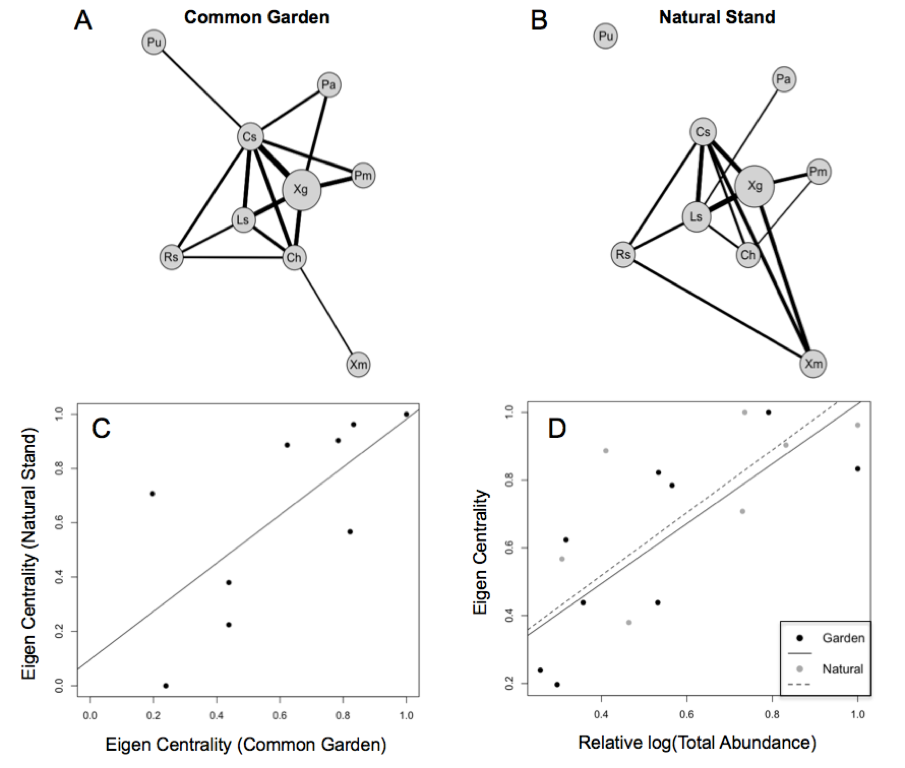
\includegraphics[width=\linewidth]{fig1}
\caption{Significant unipartite network structure was observed for
  epiphytic lichens on trees of known genotype in a common garden (ONC
  = Ogden Nature Center, Utah, USA) (A) and individual trees in a
  natural stand (Uintah, Utah, USA) (B) of the foundation species,
  \textit{Populus angustifolia}. Both networks are shown here with
  lichen species as nodes (see Methods for complete species names)
  scaled by the log of their total abundances and significant
  co-occurrence patterns between species shown as edges scaled by
  their log frequencies. The bivariate plot (C) shows the significant
  correlation in Eigen Centrality between the two networks. (D) The
  total abundance of lichen species was a significant driver of
  network structure for both networks.}
\label{fig:fig1}
\end{figure}

\begin{figure}[ht]
\centering
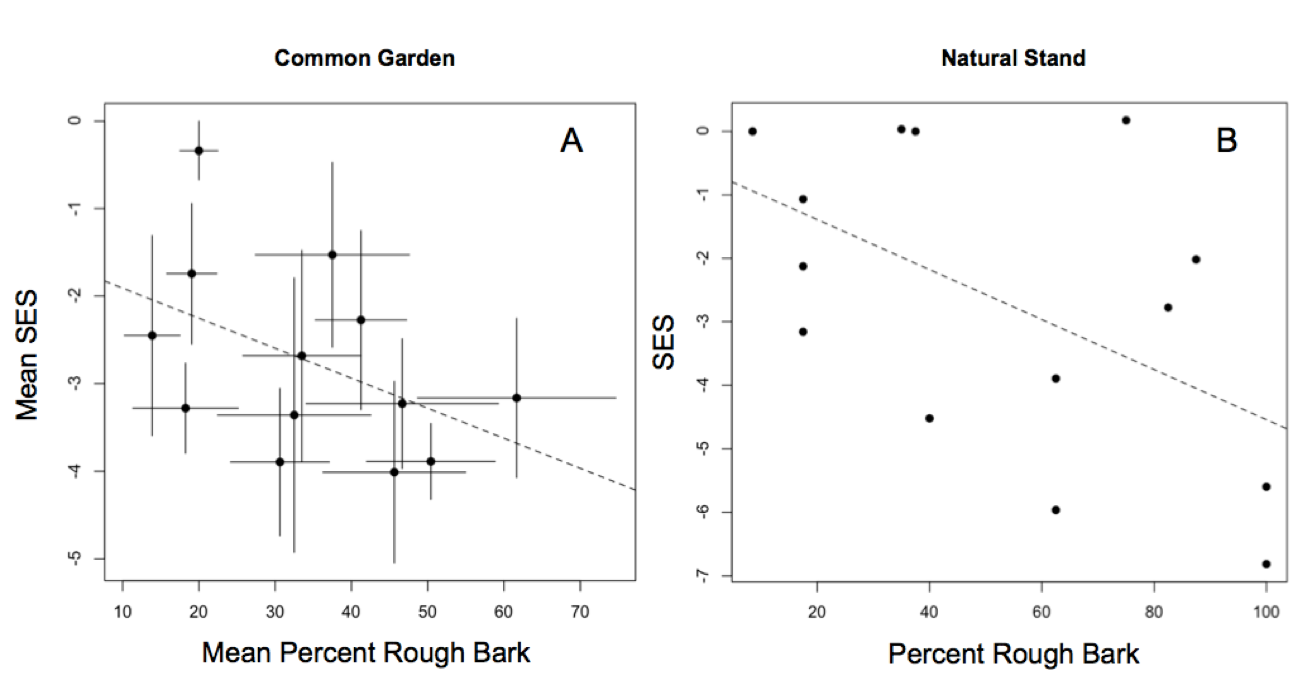
\includegraphics[width=\linewidth]{fig2}
\caption{Tree genotype influenced lichen co-occurrence patterns in the
  common garden and the natural stand through a genetically controlled
  tree trait. The lichen co-occurrence patterns were highly correlated
  with the genetically based phenotypic trait; bark roughness (i.e.,
  the percentage of textured bark), in both the common garden and
  natural stand. The scatterplot (A) shows the mean ($\pm$ 1 SE)
  percent rough bark (broadsense heritability, $H^2$ = 0.36, $\chi^2$
  = 9.214, \textit{p} = 0.002) and SES for each genotype for trees in
  the common garden with SES values becoming more negative (i.e.,
  species interactions increased), indicating stronger co-occurrence
  patterns, as bark roughness increases. The lichen communities on
  individual trees in the Unitah natural stand (B) displayed a similar
  pattern with the SES values becoming increasingly more negative on
  trees with more rough bark.}
\label{fig:fig2}
\end{figure}

\begin{figure}[ht]
\centering
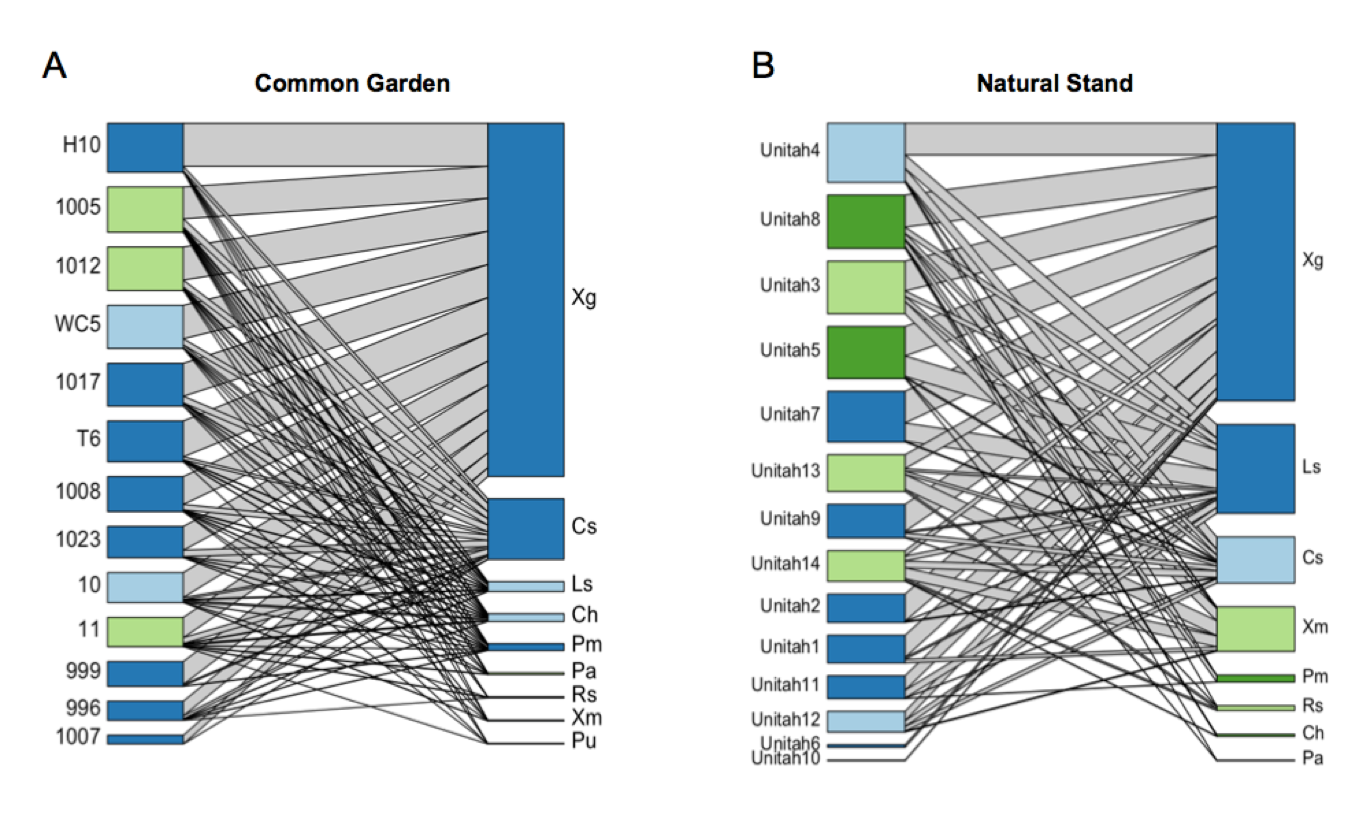
\includegraphics[width=\linewidth]{fig3}
\caption{Bipartite networks displayed significant modularity with
  modules comprised of both genotypes and species. The left most set
  of nodes shows tree genotypes (see Methods for genotype names) for
  the common garden (A) or individuals in the natural stand (B)
  connected to lichen species on the right. Both sets of nodes are
  scaled by their marginal totals (i.e., total observed individuals
  for tree nodes and total abundance for lichen species) and arranged
  by ascending totals from bottom to top. Node color shows the
  significant module membership for both trees and lichen species with
  module color having no direct relationship between the two networks,
  as modules were determined for each network independently.}
\label{fig:fig3}
\end{figure}

%% \begin{table}[ht]
%% \centering
%% \begin{tabular}{|l|l|l|}
%% \hline
%% Condition & n & p \\
%% \hline
%% A & 5 & 0.1 \\
%% \hline
%% B & 10 & 0.01 \\
%% \hline
%% \end{tabular}
%% \caption{\label{tab:example}Legend (350 words max). Example legend text.}
%% \end{table}

%% Figures and tables can be referenced in LaTeX using the ref command, e.g. Figure \ref{fig:stream} and Table \ref{tab:example}.

\end{document}
